\documentclass{beamer}
%%%%%%%%%%%%%%%%%%%%%%%%%%%%%%%%%%%%%%%%%%%%%%%%%%%%%%%%%%%%%%%%%%%%%%%%%%%%
\usepackage{amsmath}
\usepackage{amssymb}
\usepackage{amsthm}
\usepackage{fancyvrb}

\usetheme{Madrid}
%\usecolortheme{seahorse}
%\usecolortheme{rose}
\setbeamertemplate{navigation symbols}{\insertframenavigationsymbol}

\title[MCGeometry]%
{A solution to connectivity in combinatorial geometries}
%\subtitle{}

\author[SRJ, JLC, JRC]{Seth~R.~Johnson \and Jeremy~L.~Conlin \and Jesse~R.~Cheatham}

\institute[UM]{
University of Michigan, Ann Arbor
}
\date[Project presentation]{December 9, 2008}

\begin{document}
%%%%%%%%%%%%%%%%%%%%%%%%%%%%%%%%%%%%%%%%%%%%%%%%%%%%%%%%%%%%%%%%%%%%%%%%%%%%

\begin{frame}
\titlepage
\begin{center}
  
\includegraphics[width=2cm]{umlogo}
\end{center}
\end{frame}

\begin{frame}{Outline}
\tableofcontents
\end{frame}

%%%%%%%%%%%%%%%%%%%%%%%%%%%%%%%%%%%%%%%%%%%%%%%%%%%%%%%%%%%%%%%%%%%%%%%%%%%%
\section{Introduction and Background}
\subsection{La la la}
\begin{frame}
  \frametitle{Intro}
  \begin{itemize}
  \item First
  \item Second
  \item Third
\end{itemize}
\end{frame}

%%%%%%%%%%%%%%%%%%%%%%%%%%%%%%%%%%%%%%%%%%%%%%%%%%%%%%%%%%%%%%%%%%%%%%%%%%%%
\subsection{Goals}
\begin{frame}{Motivation}
\begin{columns}[c] % the "c" option specifies center vertical alignment
\column{.5\textwidth} % column designated by a command
\begin{itemize}
  \item Wish to better represent range of opacities
  \item Increasing number of groups will not increase ``opacity resolution'' at
	 transition lines
  \item Opacity Distribution Function (ODF) method allows each group to have
	 multiple opacities
  \item Implement ODFs in Milagro
  \item Improve ODF method with better frequency-dependence for improved physics
\end{itemize}

\column{.5\textwidth}
  
\includegraphics[width=\textwidth]{umlogo}
\end{columns}
\end{frame}

%%%%%%%%%%%%%%%%%%%%%%%%%%%%%%%%%%%%%%%%%%%%%%%%%%%%%%%%%%%%%%%%%%%%%%%%%%%%
\section{Implementation}
%%%%%%%%%%%%%%%%%%%%%%%%%%%%%%%%%%%%%%%%%%%%%%%%%%%%%%%%%%%%%%%%%%%%%%%%%%%%
\section{Results}
%%%%%%%%%%%%%%%%%%%%%%%%%%%%%%%%%%%%%%%%%%%%%%%%%%%%%%%%%%%%%%%%%%%%%%%%%%%%
\subsection{Complex Geometry}
\begin{frame}{Multiply connected geometry}
\begin{columns}[c]
\column{0.5\textwidth}
\begin{itemize}
  \item One cell is connected to more than once cell through the same surface
  \item Composed of sphere and four planes
\end{itemize}

\column{0.5\textwidth}
    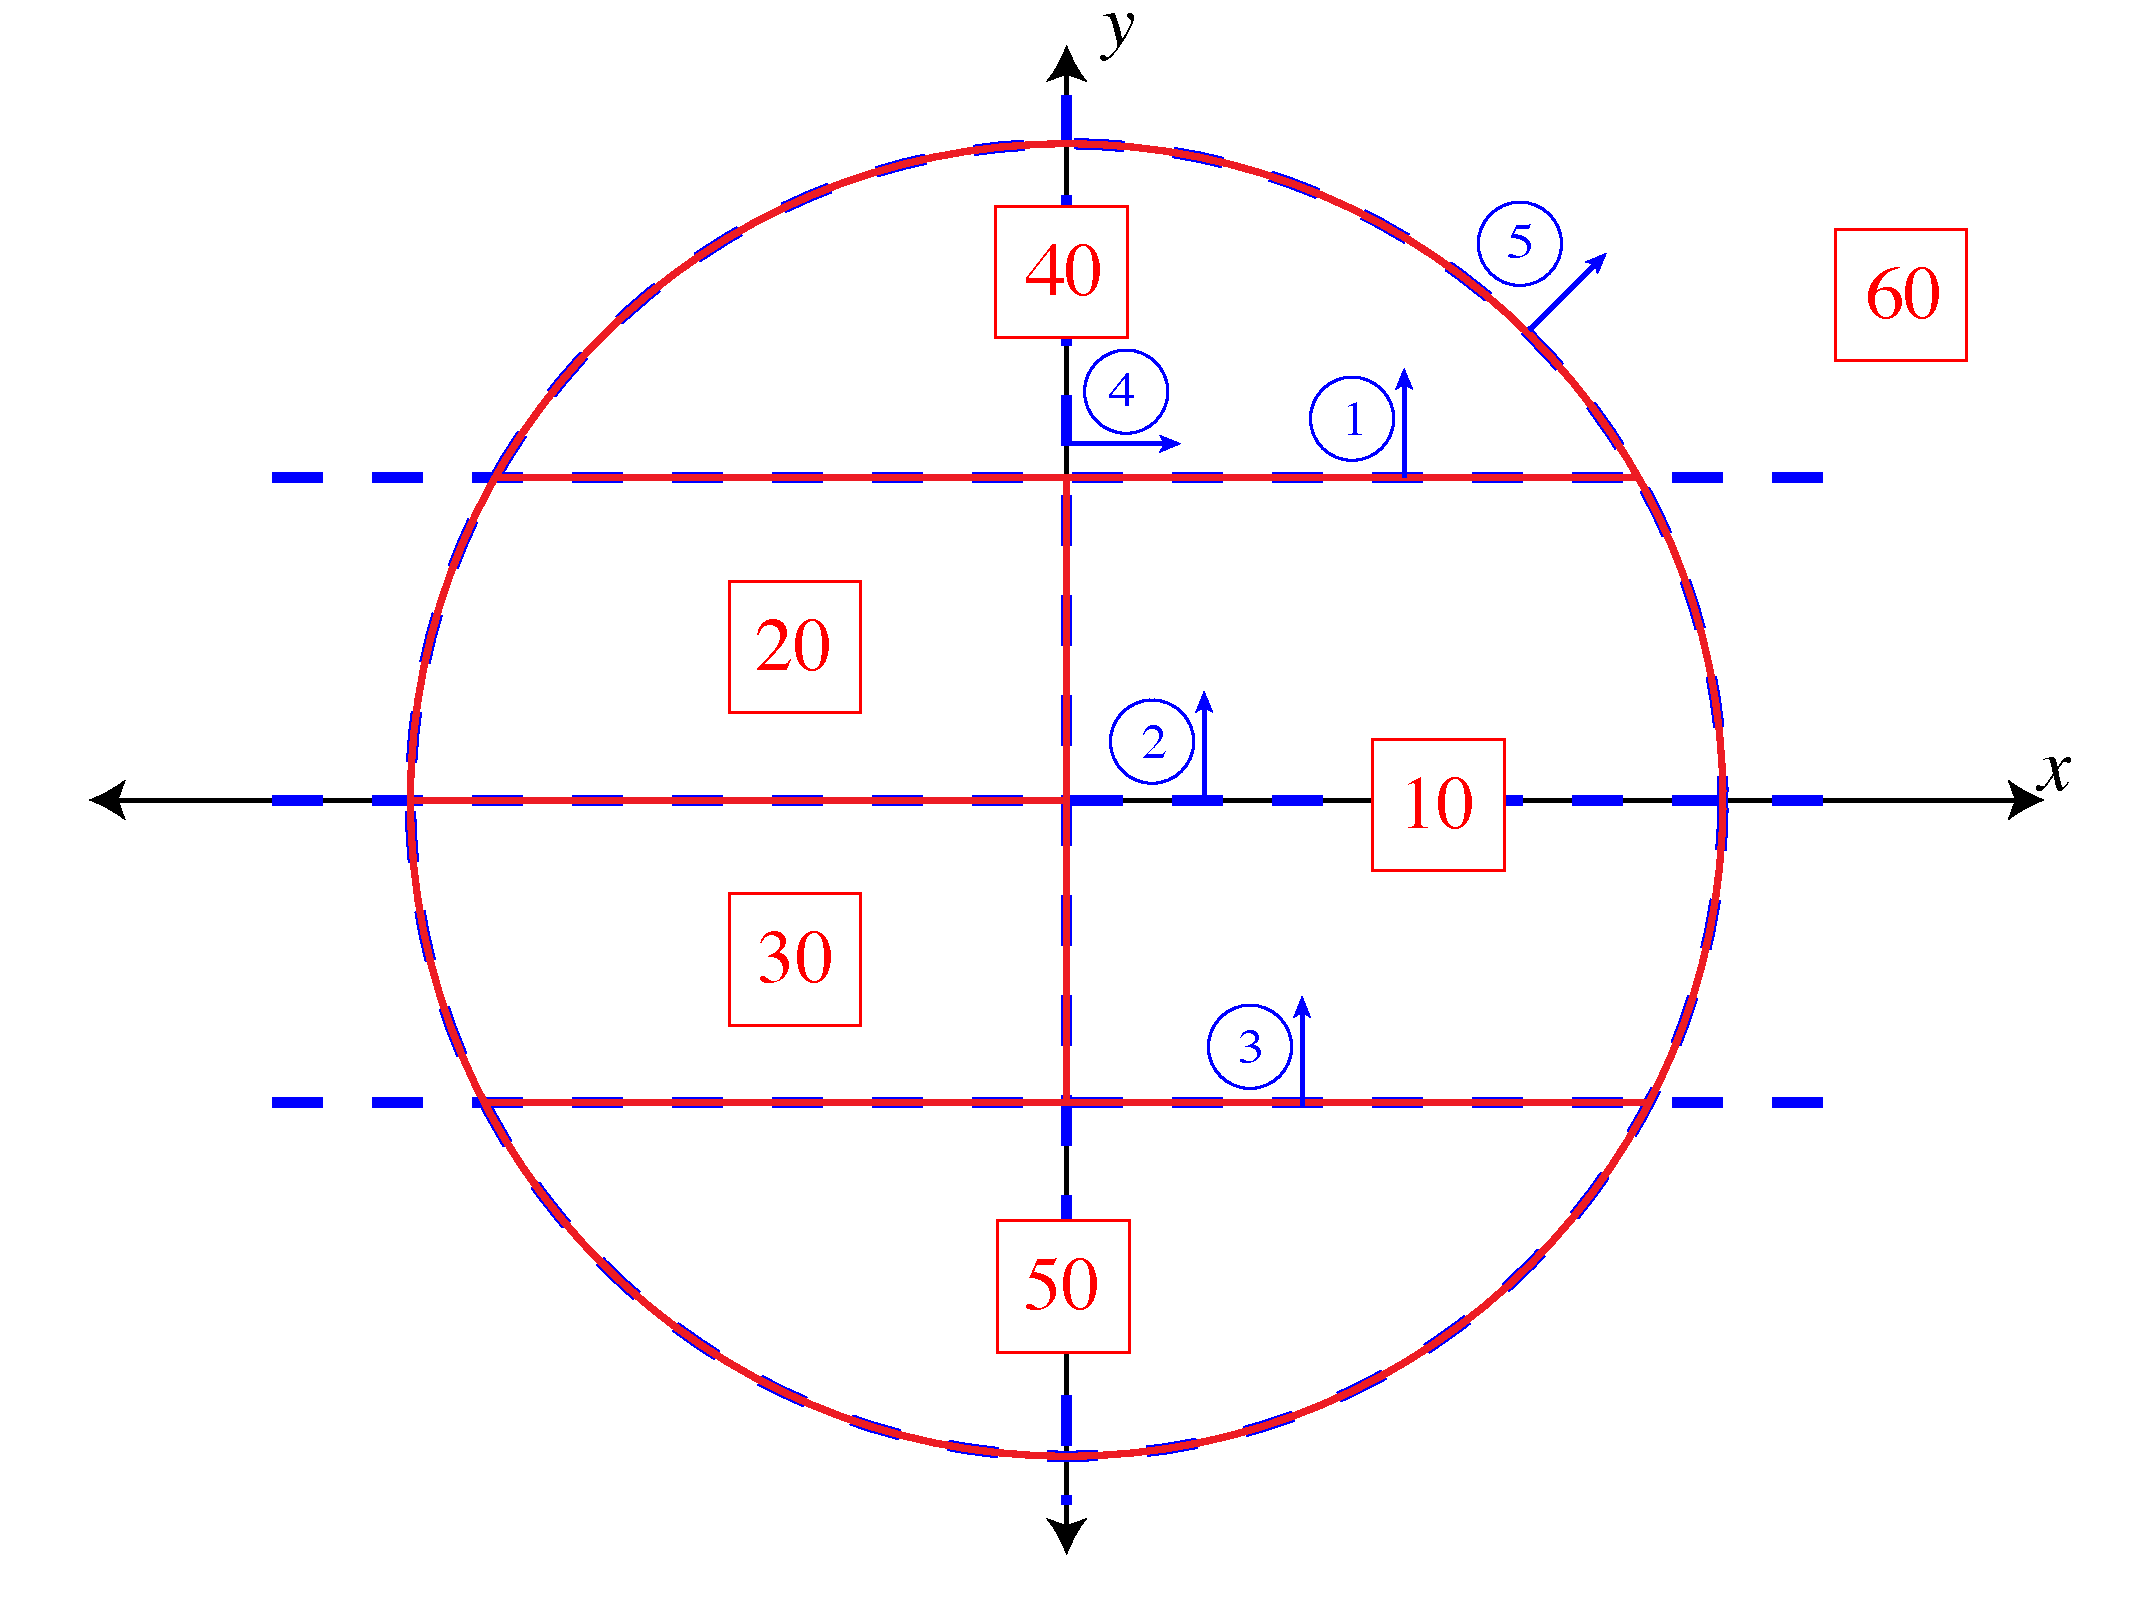
\includegraphics[width=\textwidth, keepaspectratio]{test_geom_1}
\end{columns}
\end{frame}

\begin{frame}{Complex Geometry Description}
  \begin{center}
    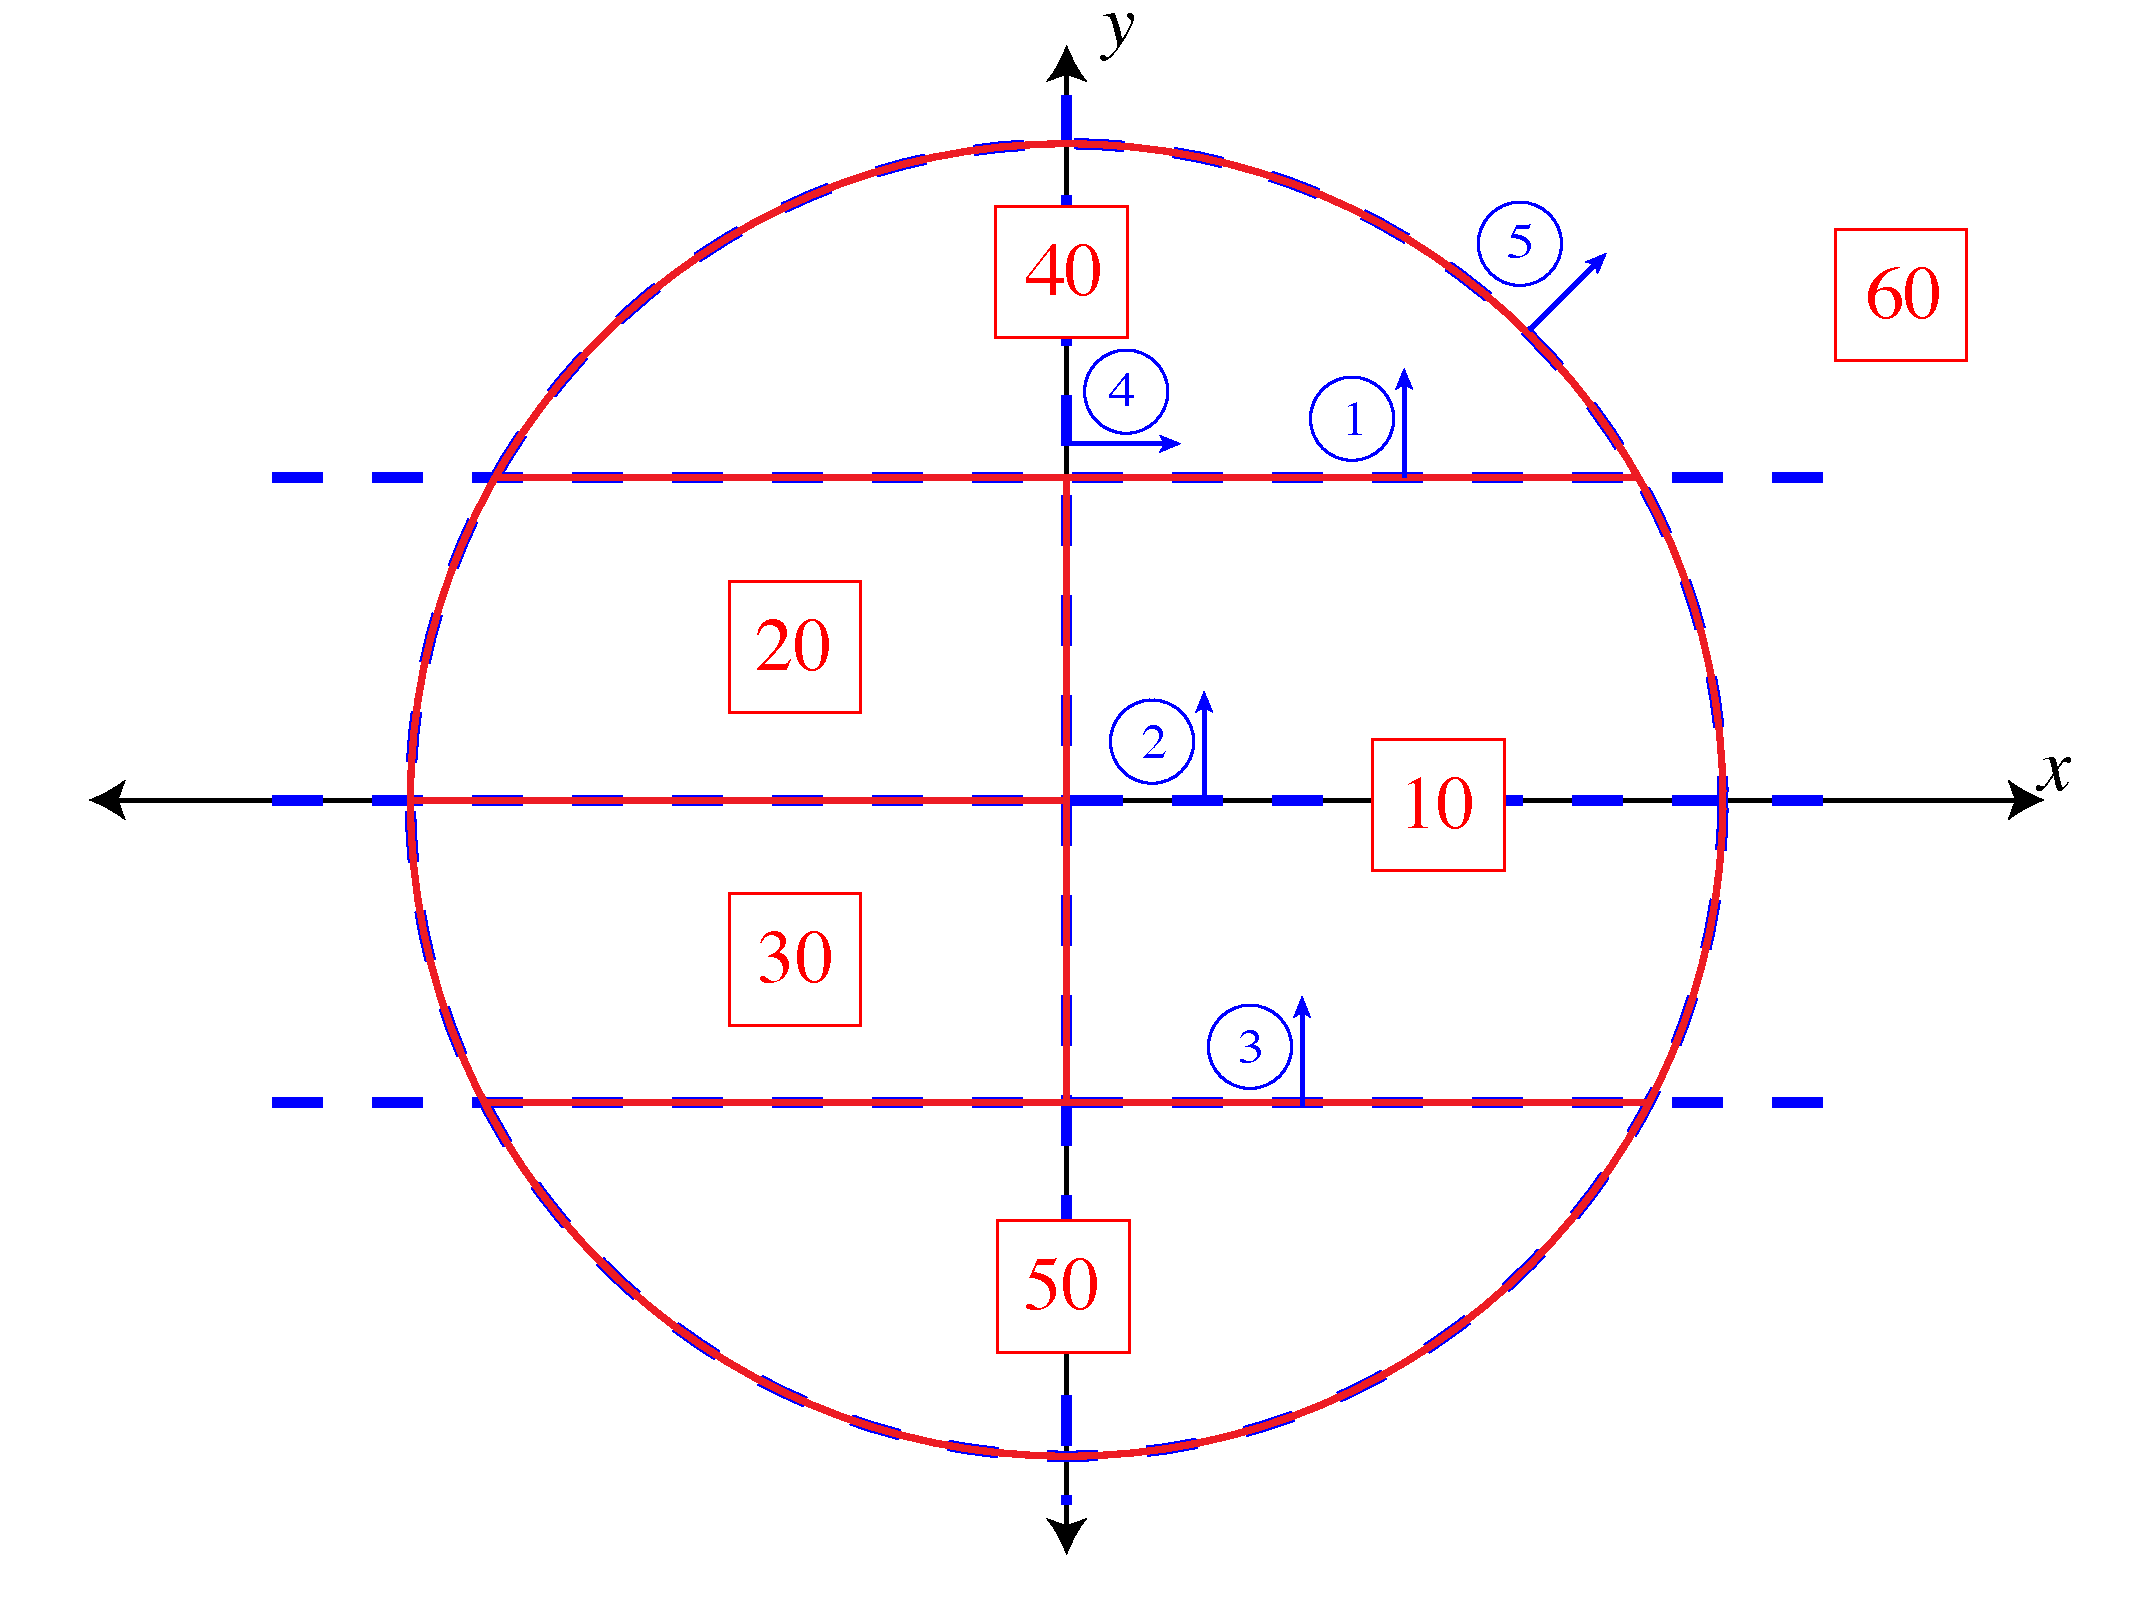
\includegraphics[width=0.9\textwidth, keepaspectratio]{test_geom_1}
  \end{center}
\end{frame}

\begin{frame}[fragile]
\frametitle{Complex Geometry Output}
\fvset{frame=single,%
		fontsize=\tiny}%

\begin{Verbatim}
SURFACES: 
 SURFACE 5: [ SPHERE Center:          <0,0,0> Radius:     3 ]
 SURFACE 1: [ PLANE  Point:           <0,1,0> Normal vector:          <0,1,0> ]
 SURFACE 2: [ PLANE  Point:           <0,0,0> Normal vector:          <0,1,0> ]
 SURFACE 3: [ PLANE  Point:           <0,-1,0> Normal vector:          <0,1,0> ]
 SURFACE 4: [ PLANE  Point:           <0,0,0> Normal vector:          <1,0,0> ]
CELLS: 
 CELL 10: -5 -1 +3 +4 
 CELL 20: -5 -1 +2 -4 
 CELL 30: -5 -2 +3 -4 
 CELL 40: -5 +1 
 CELL 50: -5 -3 
 CELL 60: -5  <NEGATED>
SURFACES TO CELLS: 
 -5: 10 20 30 40 50 
 +5: 60 
 -1: 10 20 
 +1: 40 
 -2: 30 
 +2: 20 
 -3: 50 
 +3: 10 30 
 -4: 20 30 
 +4: 10 
NEIGHBORHOOD CONNECTIVITY: 
 CELL 10: -5:{60 } -1:{40 } +3:{50 } +4:{30 20 } 
 CELL 20: -5:{60 } -1:{40 } +2:{30 } -4:{10 } 
 CELL 30: -5:{60 } -2:{20 } +3:{50 } -4:{10 } 
 CELL 40: -5:{60 } +1:{10 20 } 
 CELL 50: -5:{60 } -3:{30 10 } 
 CELL 60: -5:{50 30 10 20 40 } 
\end{Verbatim}
\end{frame}  

%%%%%%%%%%%%%%%%%%%%%%%%%%%%%%%%%%%%%%%%%%%%%%%%%%%%%%%%%%%%%%%%%%%%%%%%%%%%
\subsection{Mesh Geometry}
\begin{frame}
\frametitle{Mesh Geometry}
\begin{columns}[c]
\column{0.5\textwidth}
\begin{itemize}
    \item Mesh has $N\times N \times N$ cells
\end{itemize}

\column{0.5\textwidth}
    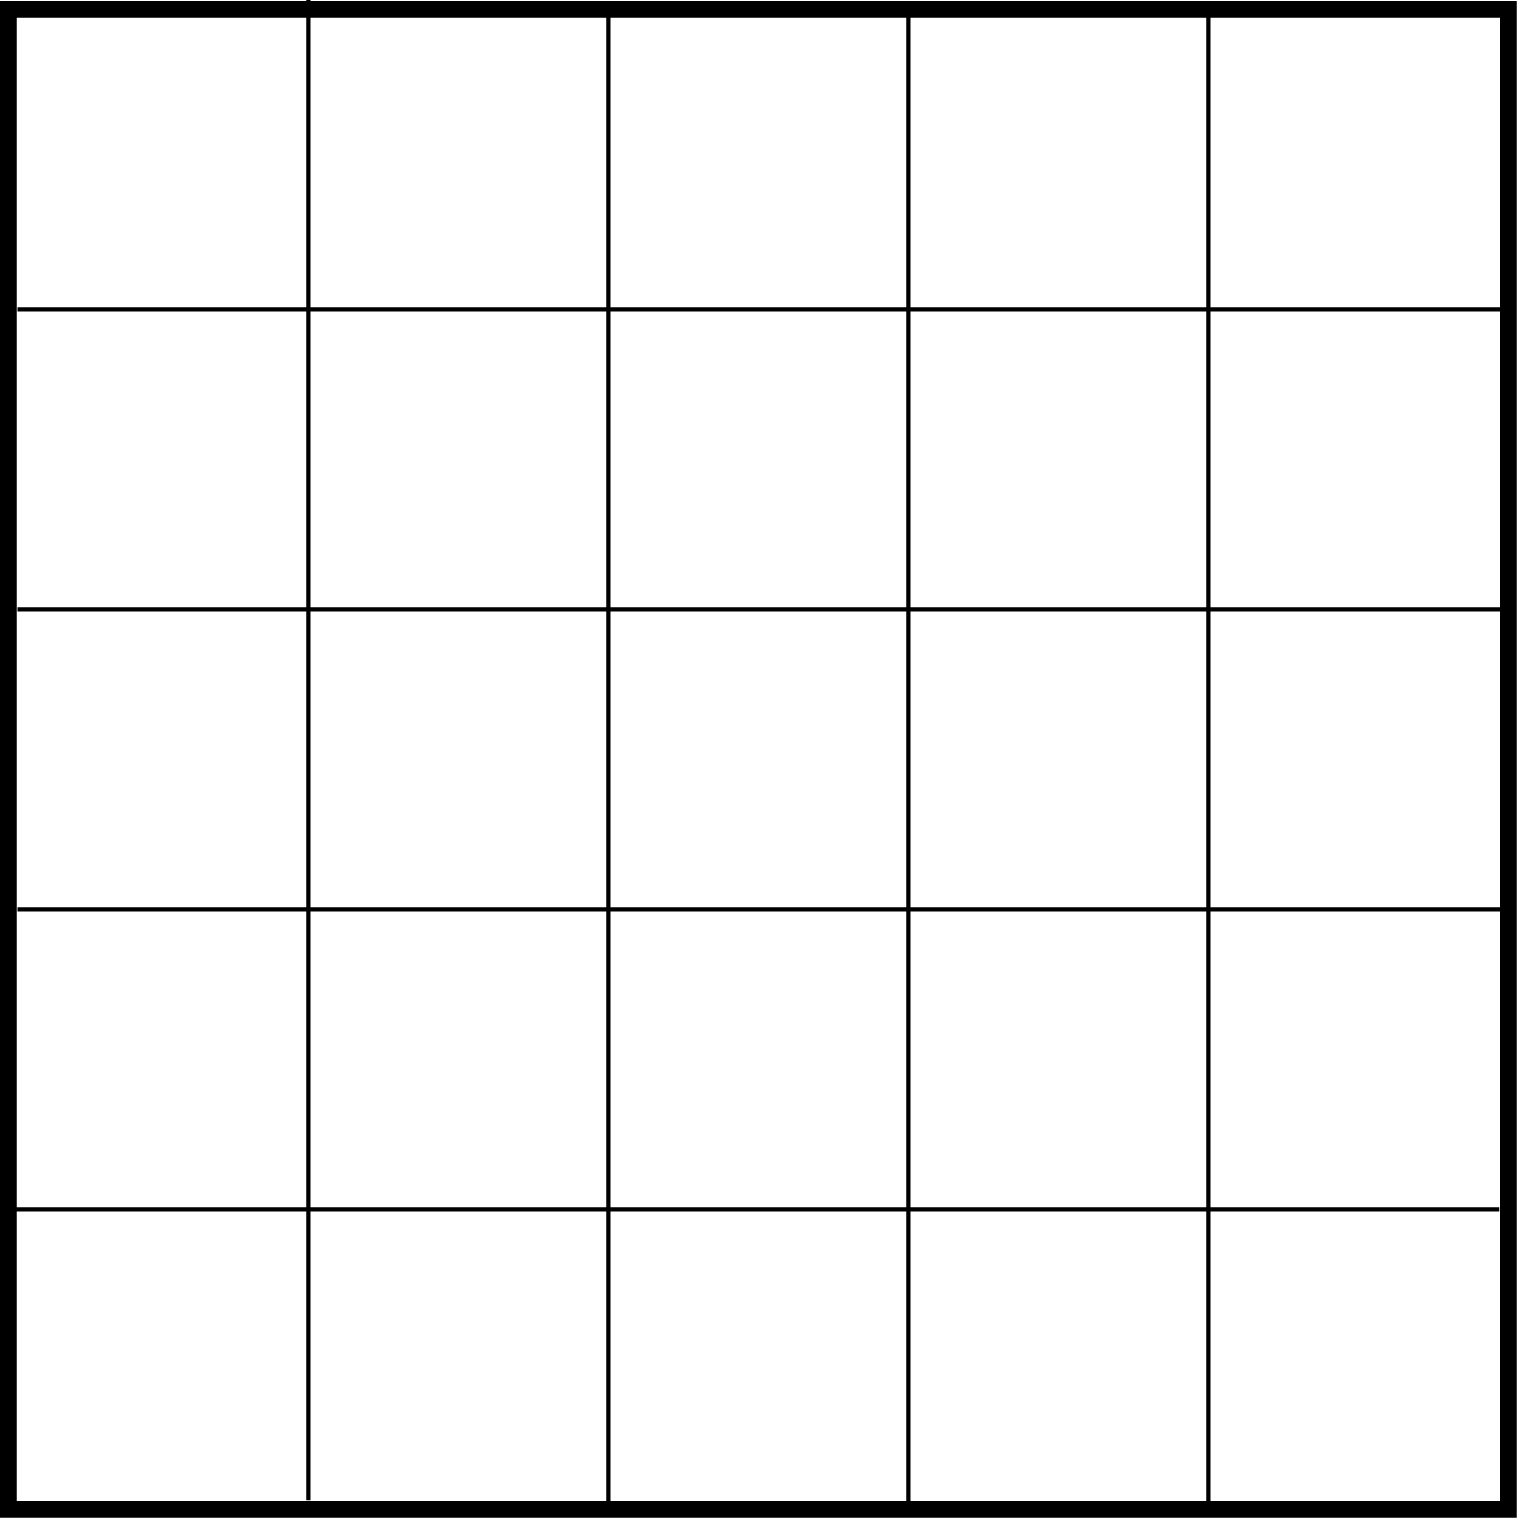
\includegraphics[width=\textwidth, keepaspectratio]{Mesh}
\end{columns}
\end{frame}

\begin{frame}
\begin{columns}[c]
\column{0.5\textwidth}
\begin{itemize}
    \item Mesh has $N\times N \times N$ cells
\end{itemize}

\column{0.5\textwidth}
    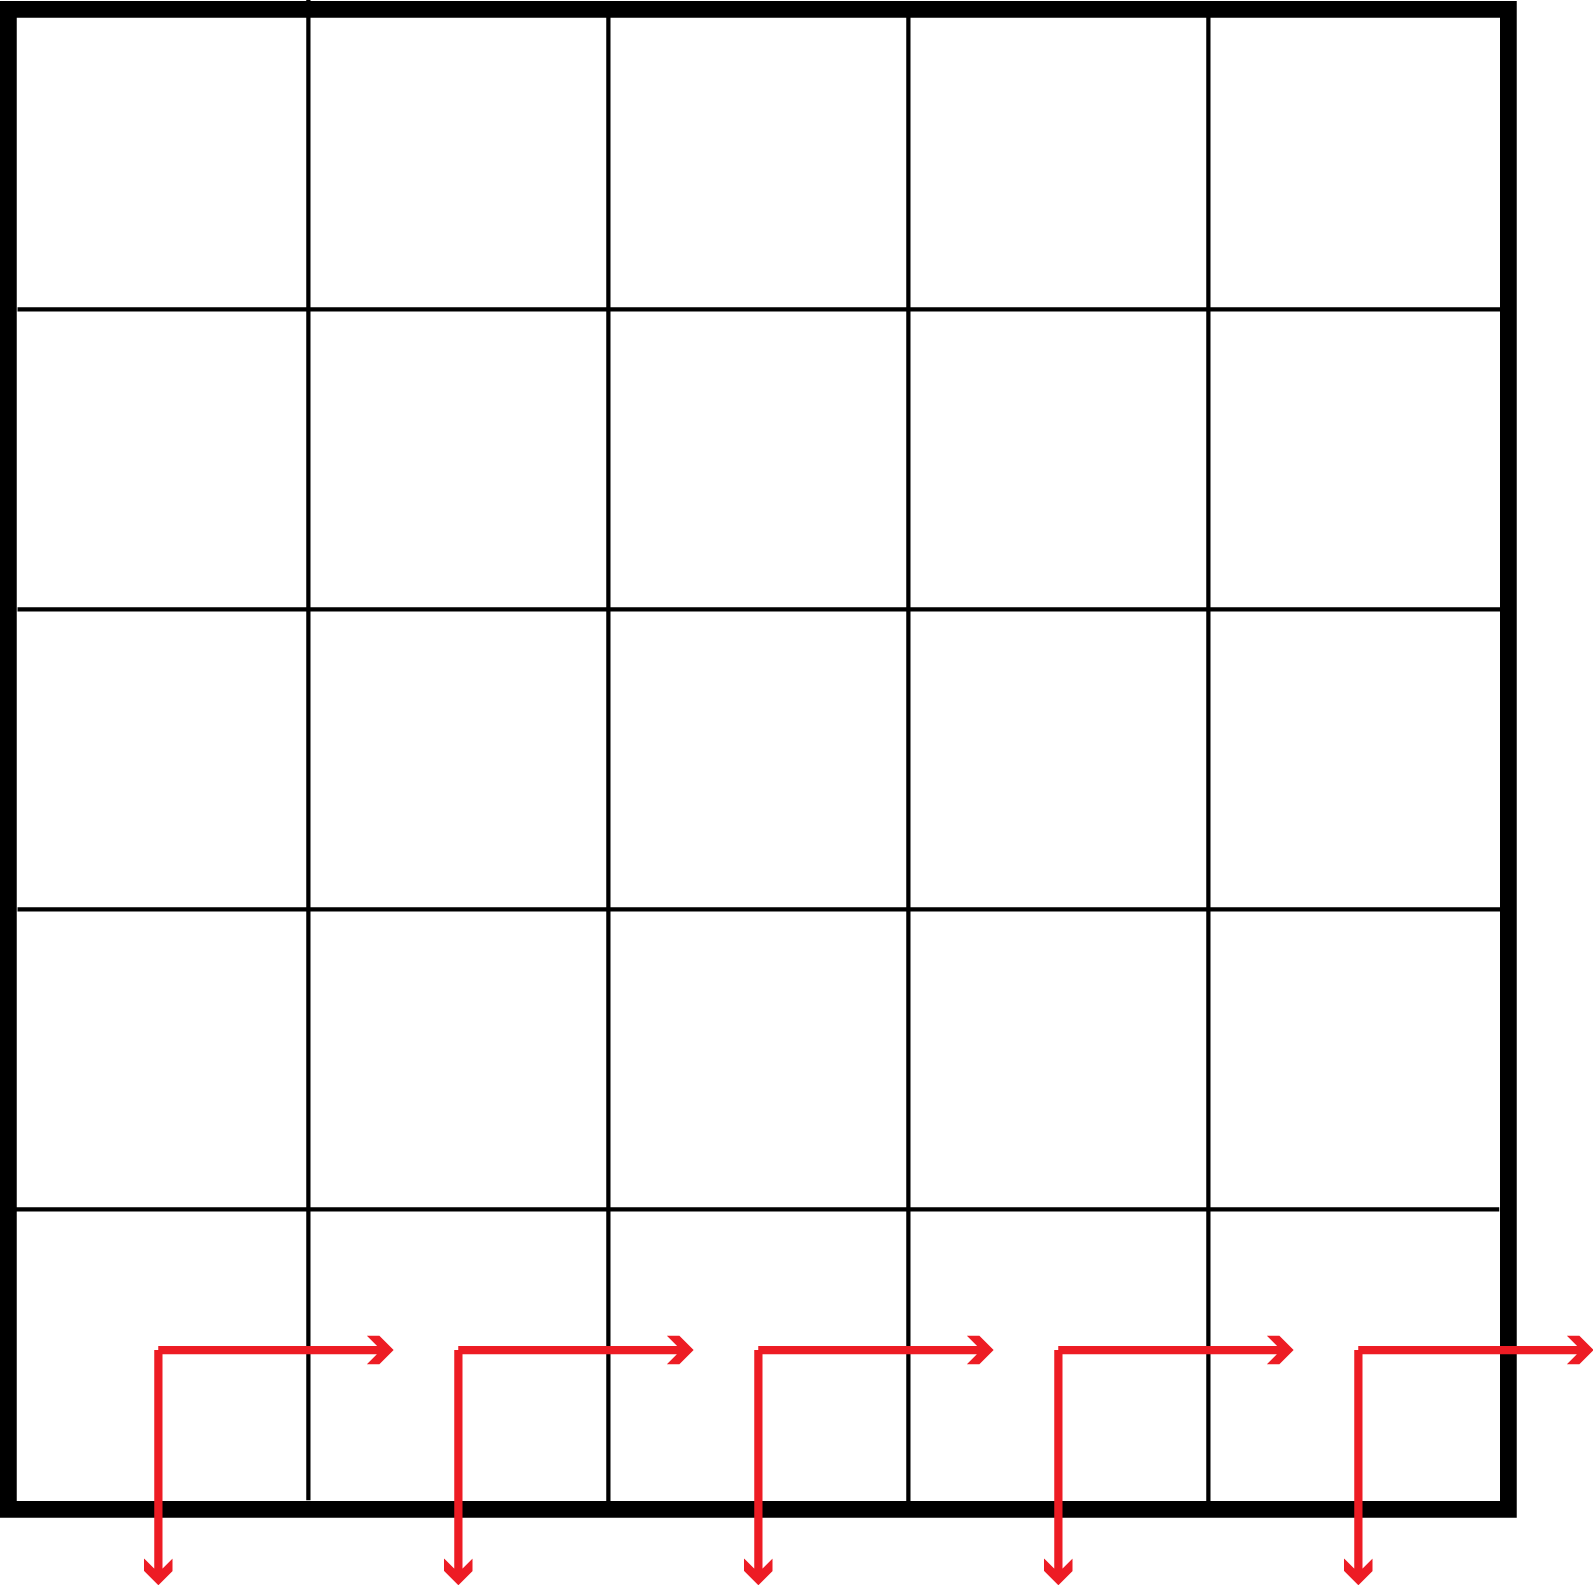
\includegraphics[width=\textwidth, keepaspectratio]{ForwardSweep}
\end{columns}
\end{frame}

\begin{frame}
\begin{columns}[c]
\column{0.5\textwidth}
\begin{itemize}
    \item Mesh has $N\times N \times N$ cells
\end{itemize}

\column{0.5\textwidth}
    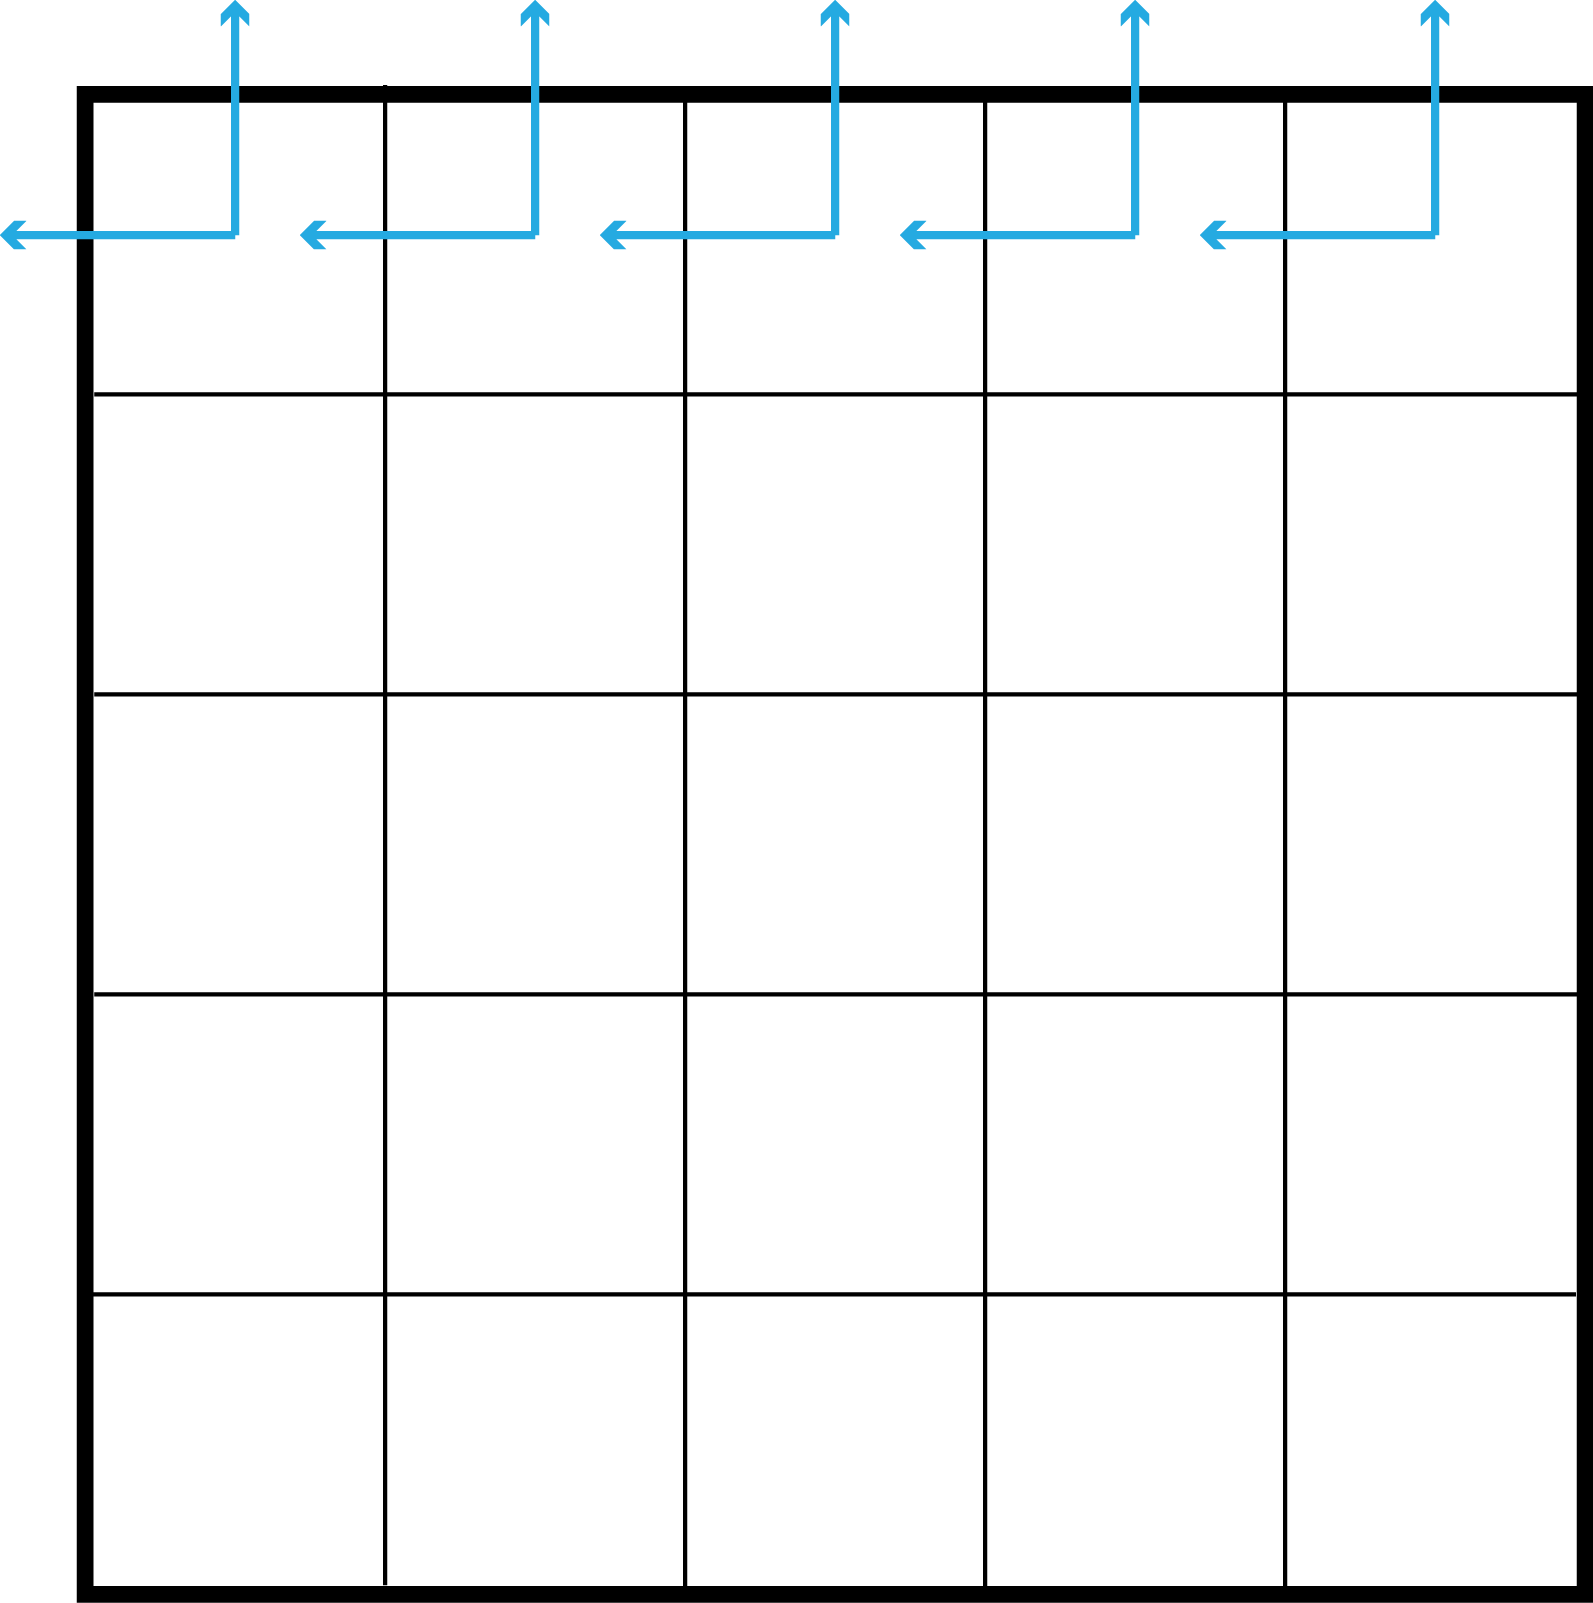
\includegraphics[width=\textwidth, keepaspectratio]{BackwardSweep}
\end{columns}
\end{frame}

\begin{frame}
    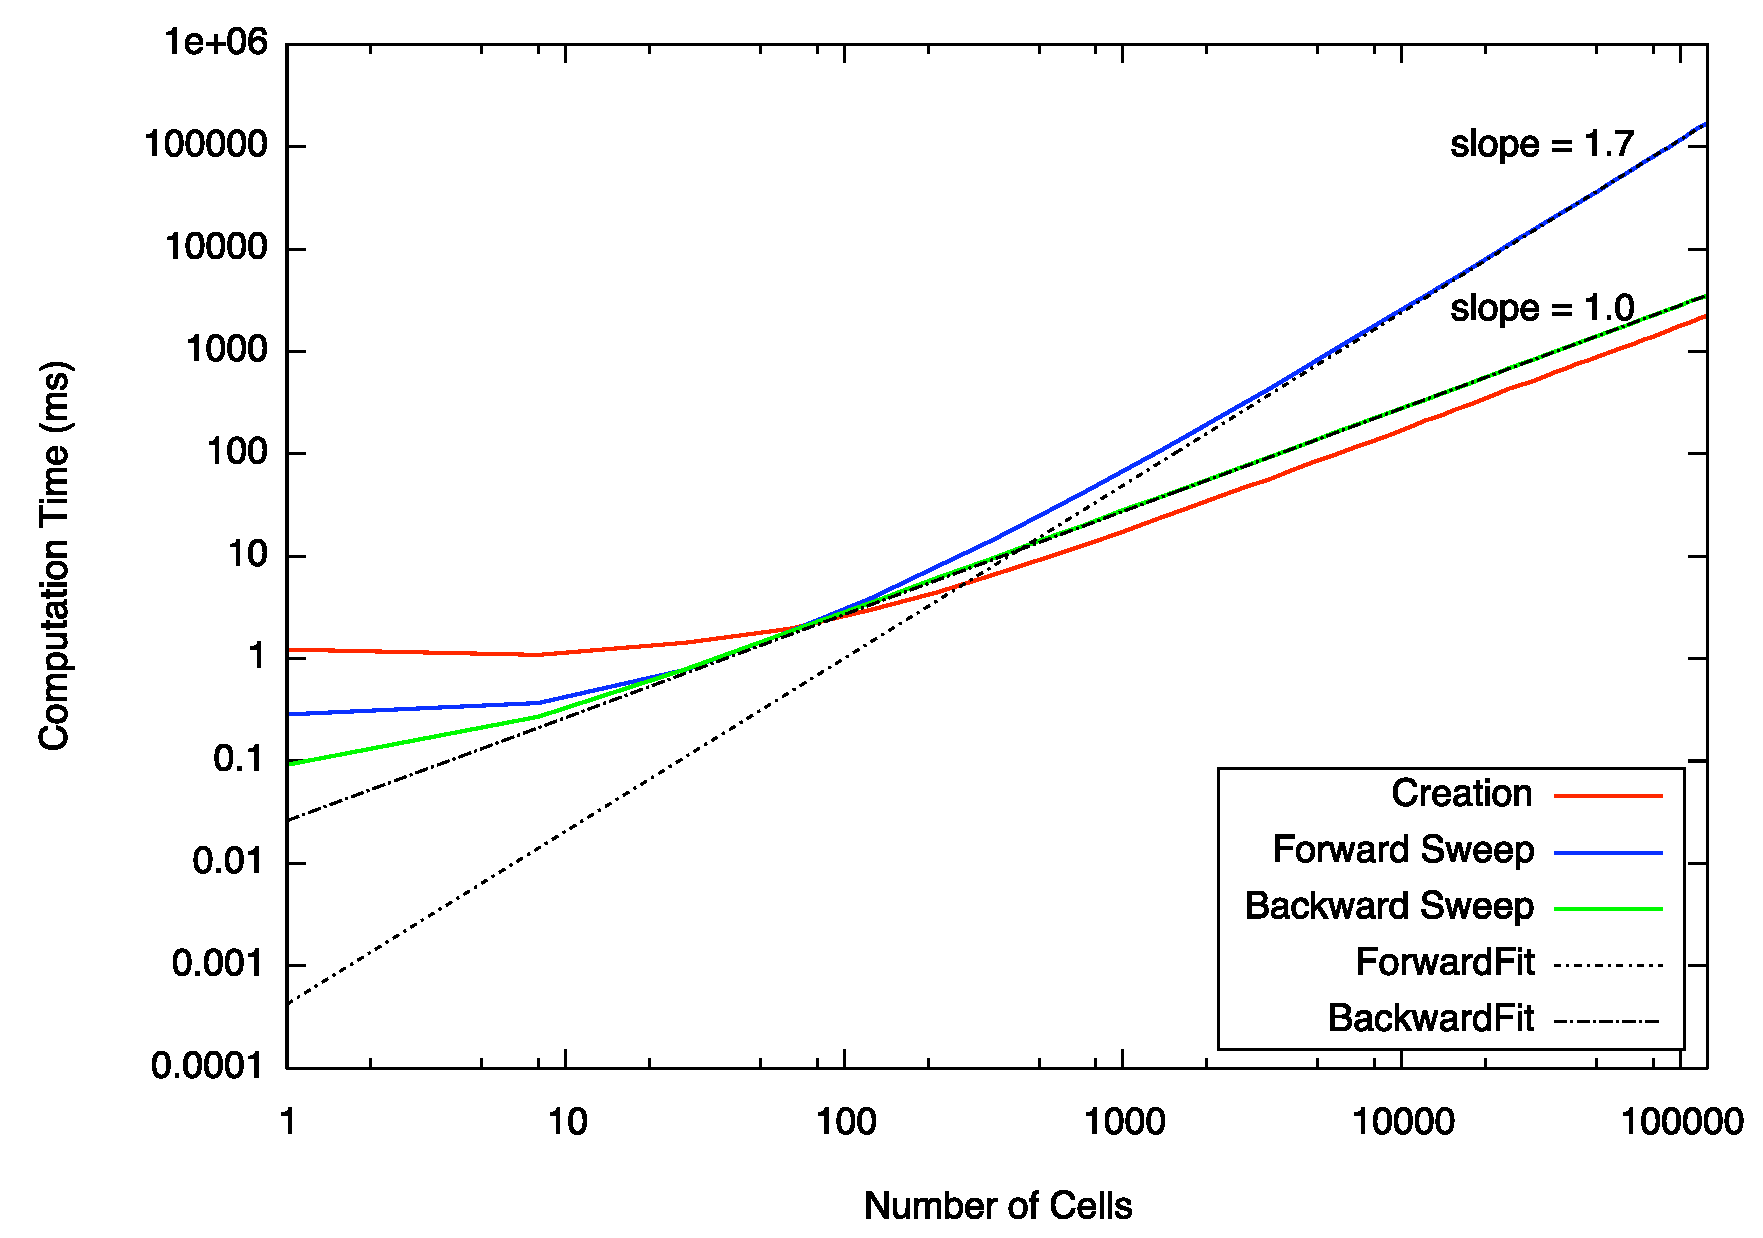
\includegraphics[width=\textwidth, keepaspectratio]{MeshTiming}
\end{frame}

\begin{frame}
\begin{columns}[c]
\column{0.5\textwidth}
\begin{itemize}
    \item Mesh has $N\times N \times N$ cells
    \item Random point picked
    \item Particle streams until it leaves geometry
\end{itemize}

\column{0.5\textwidth}
    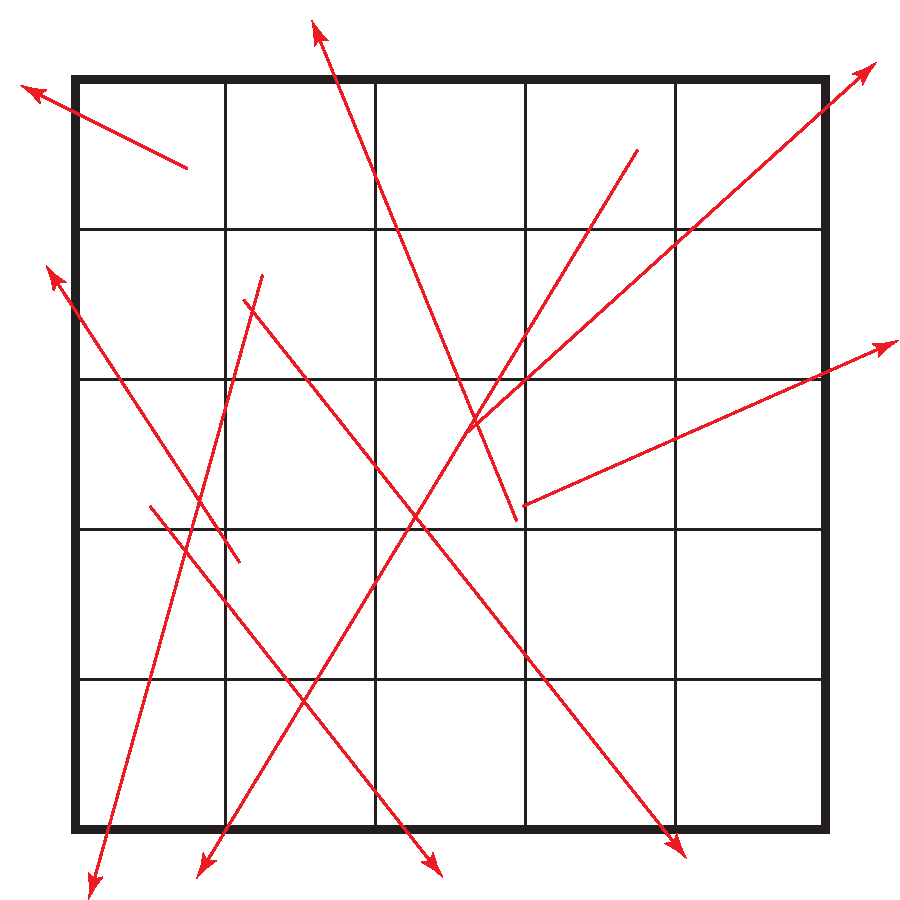
\includegraphics[width=\textwidth, keepaspectratio]{MeshCompGraphic}
\end{columns}
\end{frame}
\begin{frame}
    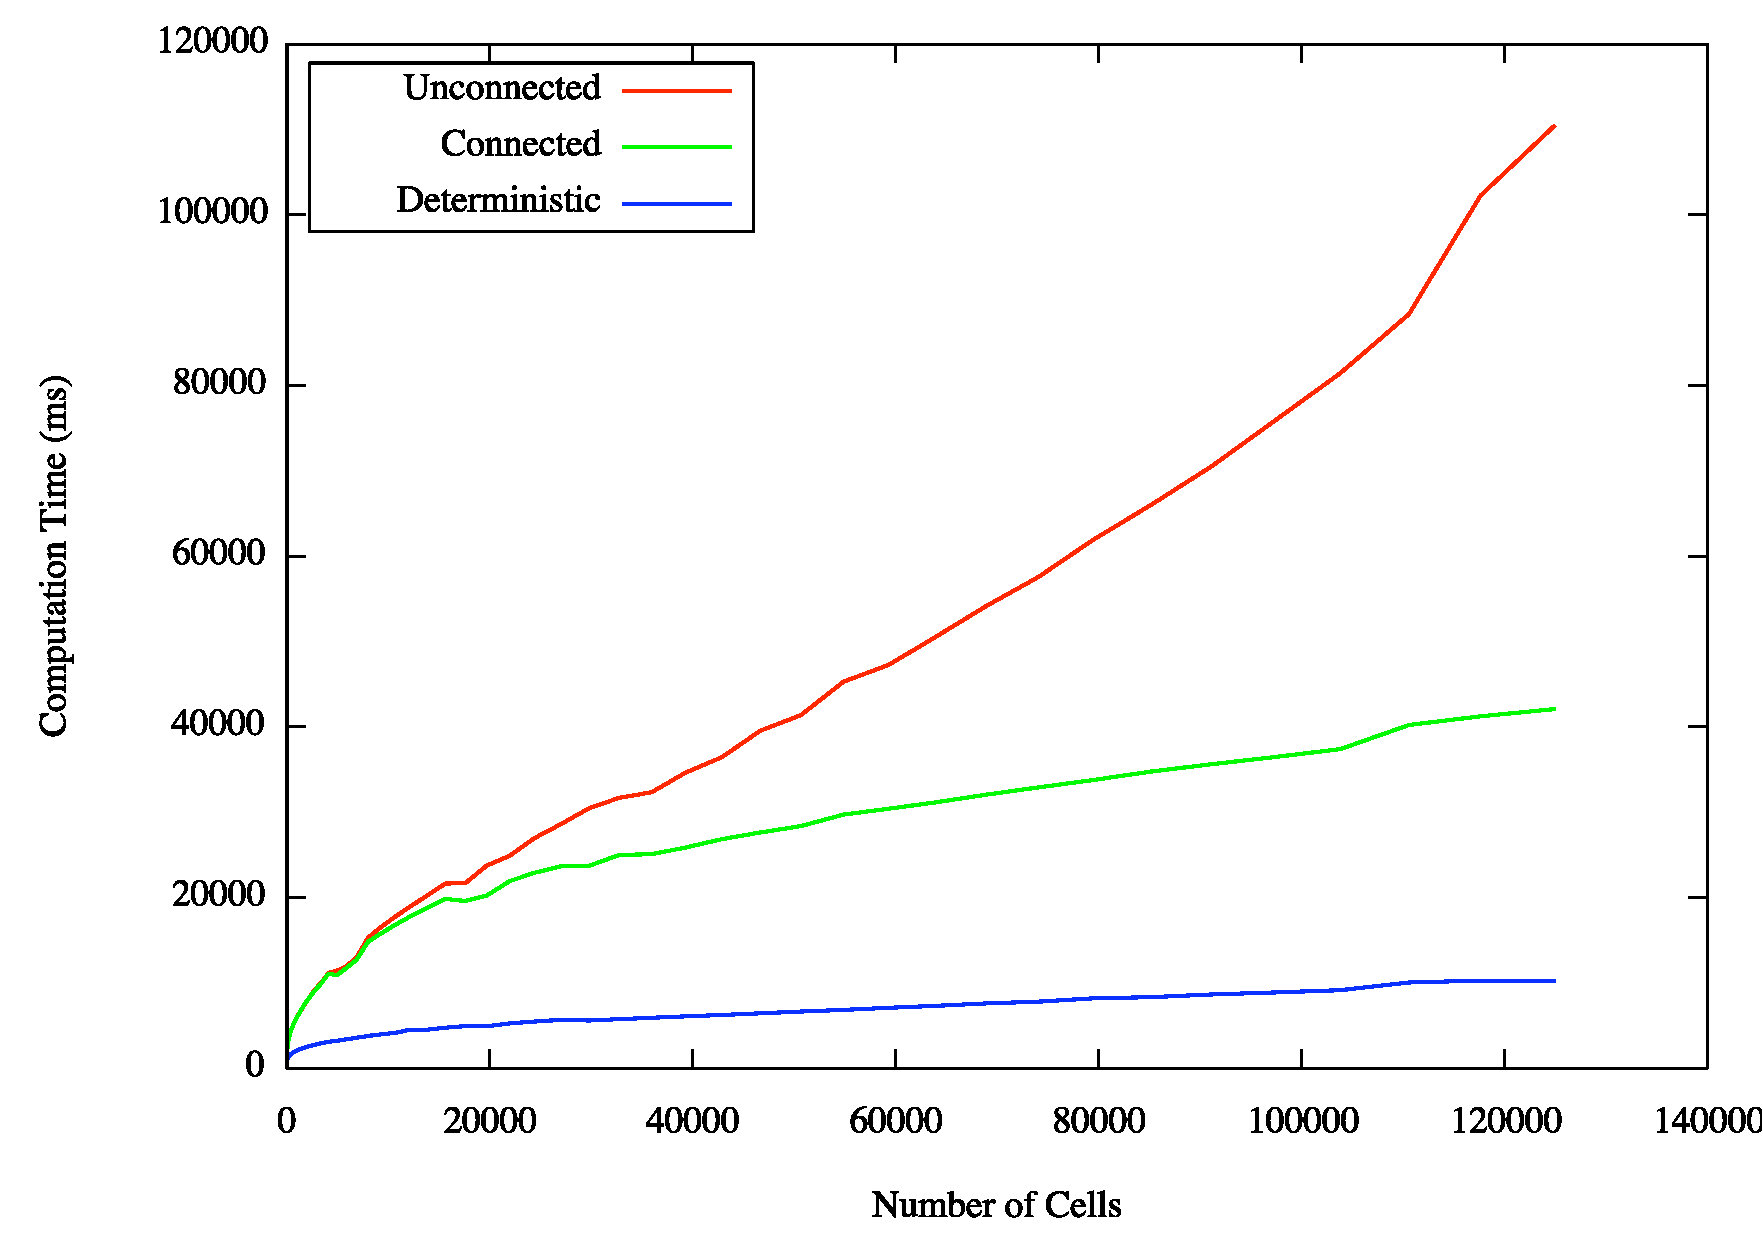
\includegraphics[width=\textwidth, keepaspectratio]{MeshComparison}
\end{frame}
%%%%%%%%%%%%%%%%%%%%%%%%%%%%%%%%%%%%%%%%%%%%%%%%%%%%%%%%%%%%%%%%%%%%%%%%%%%%
\section{Conclusions}

\begin{frame}
  \frametitle{Conclusions}
  \begin{itemize}
	 \item Our geometry works (assuming our test codes are complete)
     \item It isn't terribly difficult to implement
         \begin{itemize}
             \item We implemented the geometry code in half a semester
             \item But you don't have to!   http://code.google.com/p/mcgeometry
         \end{itemize}
     \item Caching connectivity improves runtime
     \item Better than doing the last homework assignment
         \begin{itemize}
             \item Takes more time, but …
             \item Is more useful in the long run
         \end{itemize}
	 \item We deserve an A+ (of course!)
  \end{itemize}
\end{frame}

\begin{frame}
  \frametitle{Future work}
  \begin{itemize}
	 \item Write connections to a file
	 \item Parallelism issues
   \item Further optimization tricks
  \end{itemize}
\end{frame}

%%%%%%%%%%%%%%%%%%%%%%%%%%%%%%%%%%%%%%%%%%%%%%%%%%%%%%%%%%%%%%%%%%%%%%%%%%%%
\appendix
\begin{frame}{References}
  References go here?
\end{frame}
%%%%%%%%%%%%%%%%%%%%%%%%%%%%%%%%%%%%%%%%%%%%%%%%%%%%%%%%%%%%%%%%%%%%%%%%%%%%
\end{document}
